% -*- mode: noweb; noweb-default-code-mode: R-mode; -*-
%\VignetteIndexEntry{PADOG}
%\VignetteKeywords{Gene Set Analysis, Pathway Analysis}
%\VignettePackage{PADOG}
\documentclass[11pt]{article}

%\usepackage{amsmath,epsfig,psfig,fullpage} 
\usepackage{amsmath,epsfig,fullpage} 
%\usepackage{graphicx,pstricks}
%\usepackage{ifpdf}
\usepackage[authoryear,round]{natbib}
\usepackage{hyperref}
\usepackage{url}

\parindent 0in

\bibliographystyle{abbrvnat}
\usepackage{Sweave}
\begin{document}

\title{\bf Bioconductor's PADOG package}
\author{Adi L. Tarca$^{1,2,3}$}

\maketitle

$^1$Department of Computer Science, Wayne State University\\
$^2$Bioinformatics and Computational Biology Unit of the NIH Perinatology Research Branch\\
$^3$Center for Molecular Medicine and Genetics, Wayne State University \\


%%%%%%%%%%%%%%%%%%%%%%%%%%%%%%%%%%%%%%%%%%%%%%%%%%%%%%%%%%%%%%%%%%%%%%%%%%%

\section{Overview}

This package implements the \emph{\textbf{P}athway \textbf{A}nalysis with \textbf{D}own-weighting of \textbf{O}verlapping \textbf{G}enes} (\textbf{PADOG})
 algorithm described in \cite{TarcaPADOG:2012}. The method can be applied to analyze any type of gene sets yet in here
 it is illustarted using KEGG pathways.
The method computes a gene set score as the mean of absolute values of weighted moderated gene
 \emph{t}-scores. The gene weights are chosen to favor genes appearing in few pathways versus genes
  that appear in many pathways. The significance of pathway scores is evaluated using sample/array 
  labels permutation that preserve the gene-gene correlation structure.
The package also contains a benchmark for gene set analysis in general and allows a new gene set 
analysis method to be benchmarked against PADOG or other exsisting methods (e.g. GSA).
The benchmark uses 24 different data sets, each involving a disease (e.g. Colorectal Cancer) for which there
is a KEGG pathway with the same name. The only assumption we make (proven to hold in \cite{TarcaPADOG:2012}) 
is that the KEGG's pathway with the same name as the disease under the study should be found significant 
and/or ranked near the top by gene set analysis methods when analyzing a dataset that compares normal 
with diseased samples.

\section{Pathway / gene set analysis with PADOG package}

This document provides basic introduction on how to use the {\tt PADOG} package. For extended 
description of the methods used by this package please consult \cite{TarcaPADOG:2012}.\\ 

We demonstrate the functionality of this package using a colorectal cancer dataset obtained using 
Affymetrix GeneChip technology and available 
through GEO (GSE9348) and incorporated in the {\tt KEGGdzPathwaysGEO} package. This experiment contains 12 normal samples and 70 colorectal cancer samples 
and is described in \cite{pmid20143136}. 
The RMA preprocessed data using the {\tt affy} package is the entry point for the {\tt padog} 
function:
 
\begin{Schunk}
\begin{Sinput}
> library(KEGGdzPathwaysGEO)
> library(PADOG)
> library(Biobase)
> set.seed(1)
> set="GSE9348"
> data(list=set,package="KEGGdzPathwaysGEO")
> x=get(set)
> #Extract from the dataset the required info
> exp=experimentData(x);
> dataset= exp@name
> dat.m=exprs(x)
> ano=pData(x)
> design= notes(exp)$design
> annotation= paste(x@annotation,".db",sep="")
> targetGeneSets= notes(exp)$targetGeneSets
> #run padog function on KEGG pathways
> #use NI=1000 for accurate results
> myr=padog(
+ esetm=dat.m,
+ group=ano$Group,
+ paired=design=="Paired",
+ block=ano$Block,
+ targetgs=targetGeneSets,
+ annotation=annotation,
+ gslist="KEGG.db",
+ organism="hsa",
+ verbose=FALSE,
+ Nmin=3,
+ NI=50,
+ plots=TRUE)
> myr[1:15,-c(4,5)]
\end{Sinput}
\begin{Soutput}
                                         Name    ID Size PmeanAbsT Ppadog
00230                       Purine metabolism 00230  153    0.0002  2e-04
04976                          Bile secretion 04976   71    0.0002  2e-04
00500           Starch and sucrose metabolism 00500   37    0.0600  2e-04
00062   Fatty acid elongation in mitochondria 00062    7    0.0200  2e-04
00460              Cyanoamino acid metabolism 00460    7    0.0400  2e-04
05211                    Renal cell carcinoma 05211   69    0.1800  2e-04
05212                       Pancreatic cancer 05212   69    0.2600  2e-04
03008       Ribosome biogenesis in eukaryotes 03008   70    0.0200  2e-02
04964 Proximal tubule bicarbonate reclamation 04964   23    0.1400  2e-02
05210                       Colorectal cancer 05210   62    0.1600  2e-02
04110                              Cell cycle 04110  122    0.0200  4e-02
00071                   Fatty acid metabolism 00071   42    0.1000  4e-02
00910                     Nitrogen metabolism 00910   22    0.0600  4e-02
05222                  Small cell lung cancer 05222   85    0.1600  4e-02
05223              Non-small cell lung cancer 05223   54    0.2600  4e-02
\end{Soutput}
\end{Schunk}
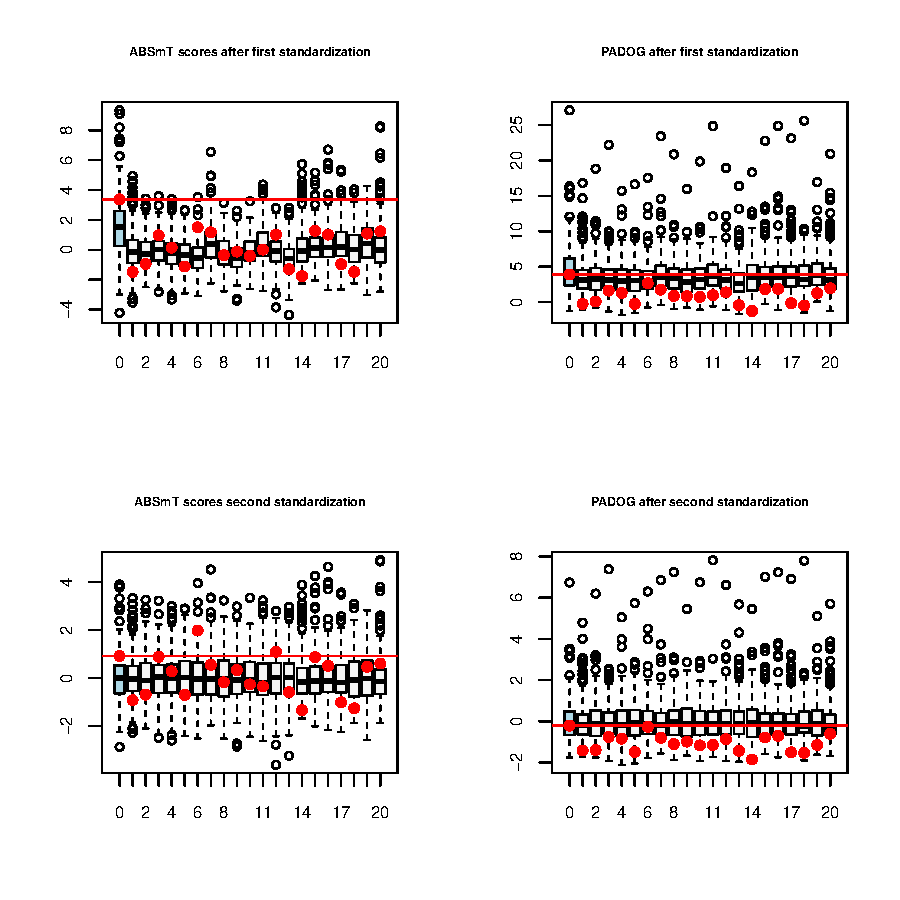
\includegraphics{PADOG-fig1}

Note that for this colorectal cancer dataset it is reasonbale to expect that the KEGG's Colorectal cancer pathway 
will be found significant and/or ranked close to the top. PmeanAbsT corresponds to the p-value
obtained without using gene weights and hence the result is worse (higher p-value) compared to Ppadog obtained by 
using the gene weights that are inversly related to how often the genes apear accross all gene sets to be analyzed.
The plot created when {\tt plots=TRUE} in the call to {\tt padog} shows how gene weighting 
improves the gene set analysis for the traget pathway set via the {\tt targetgs} argument. Figure above shows 
the distribution of pathway/gene set scores (\emph{y} axis)
for PADOG and ABSmT (which is PADOG without weights) after the first standardization (row randomization) and 
after second standardization (between gene sets standardization). The \emph{x} axis 
represents the number of iterations. Iteration 0 uses true class labels, all others used randomly permuted 
labels. The target pathway (set via the {\tt targetgs} argument) in this dataset is the 
\emph{Colorectal Cancer pathway} (KEGG ID 05210). Its score 
is shown with a red bullet throughout all 4 panels, and a red horizontal line marks its level when obtained 
with the true class labels ($ite=0$, x-axis). The box plots of scores obtained with the true class labels 
are also highlighted in blue. With PADOG, after the second standardization, the target pathway scores 
obtained from permutations are less frequently above the red line ($0/20$) (more extreme) than for ABSmT 
 ($5/20$). Over 1,000 iterations, $p_{PADOG}$ was estimated to be 0.013 while $p_{ABSmT}$ worse, i.e. 0.135.


\section{Benchmark of gene set analysis methods}

The entire collection of 24 datasets available in {\tt KEGGdzPathwaysGEO} package that can be used to benchmark PADOG 
against existing approaches is given in Table \ref{tab:datasets}:

\begin{table}
\caption{\bf{The 24 datasets used in the benchmark of pathway analysis methods}}
\begin{tabular}{rllllll}
  \hline
 GEOID&Pubmed& Ref.& Disease/Target pathway & KEGGID & Tissue \\
  \hline
GSE1297&14769913&\cite{pmid14769913}& Alzheimer's Disease& hsa05010 &Hippocampal CA1\\
GSE5281&17077275&\cite{pmid17077275}& Alzheimer's Disease& hsa05010 &Brain, Entorhinal Cortex\\
GSE5281&17077275&\cite{pmid17077275}& Alzheimer's Disease& hsa05010 &Brain, hippocampus\\
GSE5281&17077275&\cite{pmid17077275}& Alzheimer's Disease& hsa05010 &Brain, Primary visual cortex\\
GSE20153&20926834&\cite{pmid20926834}& Parkinson's disease&hsa05012&Lymphoblasts\\
GSE20291&15965975&\cite{pmid15965975}& Parkinson's disease&hsa05012 &Postmortem brain putamen\\
GSE8762&17724341&\cite{pmid17724341}& Huntington's disease&hsa05016&Lymphocytes (blood) \\
GSE4107&17317818&\cite{pmid17317818}& Colorectal Cancer& hsa05210&Mucosa\\
GSE8671&18171984&\cite{pmid18171984}& Colorectal Cancer& hsa05210&Colon\\
GSE9348&20143136&\cite{pmid20143136}& Colorectal Cancer& hsa05210&Colon\\
GSE14762&19252501 &\cite{pmid19252501}& Renal Cancer& hsa05211&Kidney \\
GSE781&14641932&\cite{pmid14641932}& Renal Cancer& hsa05211&Kidney\\
GSE15471&19260470&\cite{pmid19260470}& Pancreatic Cancer& hsa05212&Pancreas\\
GSE16515&19732725&\cite{pmid19732725}& Pancreatic Cancer& hsa05212&Pancreas\\
GSE19728&&-&Glioma&hsa05214 &Brain\\
GSE21354&&-&Glioma&hsa05214 &Brain, Spine\\
GSE6956&18245496&\cite{pmid18245496}&Prostate Cancer& hsa05215 &Prostate\\
GSE6956&18245496&\cite{pmid18245496}& Prostate Cancer& hsa05215&Prostate\\
GSE3467&16365291&\cite{pmid16365291}& Thyroid Cancer& hsa05216&Thyroid\\
GSE3678&&-&Thyroid Cancer&hsa05216& Thyroid \\
GSE9476&17910043&\cite{pmid17910043}& Acute myeloid leukemia&hsa05221&Blood, Bone marrow \\
GSE18842&20878980&\cite{pmid20878980}& Non-Small Cell Lung Cancer&hsa05223&Lung \\
GSE19188&20421987&\cite{pmid20421987}& Non-Small Cell Lung Cancer&hsa05223&Lung \\
GSE3585&17045896&\cite{pmid17045896}& Dilated cardiomyopathy&hsa05414 &Heart\\
   \hline
\end{tabular}

\begin{flushleft} The 24 datasets used to compare the pathway analysis methods were obtained from GEO.
\end{flushleft}
\label{tab:datasets}
\end{table}

To illustrate how to compare PADOG against a user defined gene set analysis method we create a function called 
{\tt randomF} that assignes random uniform P-values to gene sets. The user defined function has to take in 3 arguments:
\begin{enumerate}
\item {\tt set}: the name of a dataset available in from the KEGGdzPathwaysGEO package;
\item {\tt mygslist}: a list with elements being vectors of gene ids for a given geneset
\item {\tt minsize}: minimum number of genes in a geneset to be considered for analysis
\end{enumerate}
 
The output should be a dataframe with columns: ID, P, Rank, Dataset, Method for the geneset(s) considered to be relevant 
in that dataset (targetGeneSets).  

\begin{Schunk}
\begin{Sinput}
> randomF=function(set,mygslist,minsize){
+ set.seed(1)
+ #this loads the dataset in an ExpressionSet object called x
+ data(list=set,package="KEGGdzPathwaysGEO")
+ x=get(set)
+ 
+ #Extract from the dataset the required info to be passed to padog
+ exp=experimentData(x);
+ dat.m=exprs(x)
+ ano=pData(x)
+ dataset= exp@name
+ design= notes(exp)$design
+ annotation= paste(x@annotation,".db",sep="")
+ targetGeneSets= notes(exp)$targetGeneSets
+ 
+ 
+ #get rid of duplicates probesets per ENTREZ ID by keeping the probeset 
+ #with smallest p-value (computed using limma) 
+ aT1=filteranot(esetm=dat.m,group=ano$Group,paired=(design=="Paired"),
+  block=ano$Block,annotation=annotation)
+ #create an output dataframe for this toy method with random gene set p-values
+ mygslistSize=unlist(lapply(mygslist,function(x){length(intersect(aT1$ENTREZID,x))}))
+ res=data.frame(ID=names(mygslist),P=runif(length(mygslist)),
+  Size=mygslistSize,stringsAsFactors=FALSE)
+ res$FDR=p.adjust(res$P,"fdr")
+ #drop genesets with less than minsize genes in the current dataset 
+ res=res[res$Size>=minsize,]
+ #compute ranks
+ res$Rank=rank(res$P)/dim(res)[1]*100
+ #needed to compare ranks between methods; must be the same as given 
+ #in mymethods argument "list(myRand="
+ res$Method="myRand";
+ #needed because comparisons of ranks between methods is paired at dataset level
+ res$Dataset<-dataset;
+ #output only result for the targetGeneSets 
+ #which are gene sets expected to be relevant in this dataset
+ return(res[res$ID %in% targetGeneSets,])
+ }
> #run the analysis on all 24 datasets and compare the new method "myRand" with 
> #PADOG and GSA (if installed) (chosen as reference since is listed first in the existingMethods)
> #if the package parallel is installed datasets are analyzed in parallel.
> #out=compPADOG(datasets=NULL,existingMethods=c("GSA","PADOG"),
>  #mymethods=list(myRand=randomF),
>  #gslist="KEGG.db",Nmin=3,NI=1000,plots=FALSE,verbose=FALSE,use.parallel=TRUE,dseed=1,pkgs=c("GSA","PADOG"))
> 
> #compare myRand against PADOG on 4 datasets only
> #mysets=data(package="KEGGdzPathwaysGEO")$results[,"Item"]
> mysets=c("GSE9348","GSE8671","GSE1297")
> out=compPADOG(datasets=mysets,existingMethods=c("PADOG"),
+  mymethods=list(myRand=randomF),
+  gslist="KEGG.db",Nmin=3,NI=40,plots=TRUE,verbose=FALSE,use.parallel=FALSE,dseed=1,pkgs=NULL)
> print(out)
\end{Sinput}
\begin{Soutput}
$summary
       Method   p geomean     p med % p.value<0.05 % q.value<0.05 rank mean
PADOG   PADOG 0.001160397   0.00025            100          66.67  4.279908
myRand myRand   0.1675201 0.5995658          33.33              0  39.97116
       rank med p Wilcox.     p LME coef. LME
PADOG  4.867257     1.000 1.0000000   0.00000
myRand 59.73451     0.875 0.8476676  35.69125

$ranks
$ranks$PADOG
[1] 1.777778 6.194690 4.867257

$ranks$myRand
[1]  0.4444444 59.7345133 59.7345133


$pvalues
$pvalues$PADOG
[1] 0.00025 0.00025 0.02500

$pvalues$myRand
[1] 0.01307758 0.59956583 0.59956583


$qvalues
$qvalues$PADOG
[1] 0.008035714 0.003766667 0.513636364

$qvalues$myRand
[1] 0.9691438 0.9691438 0.9691438
\end{Soutput}
\begin{Sinput}
> 
\end{Sinput}
\end{Schunk}
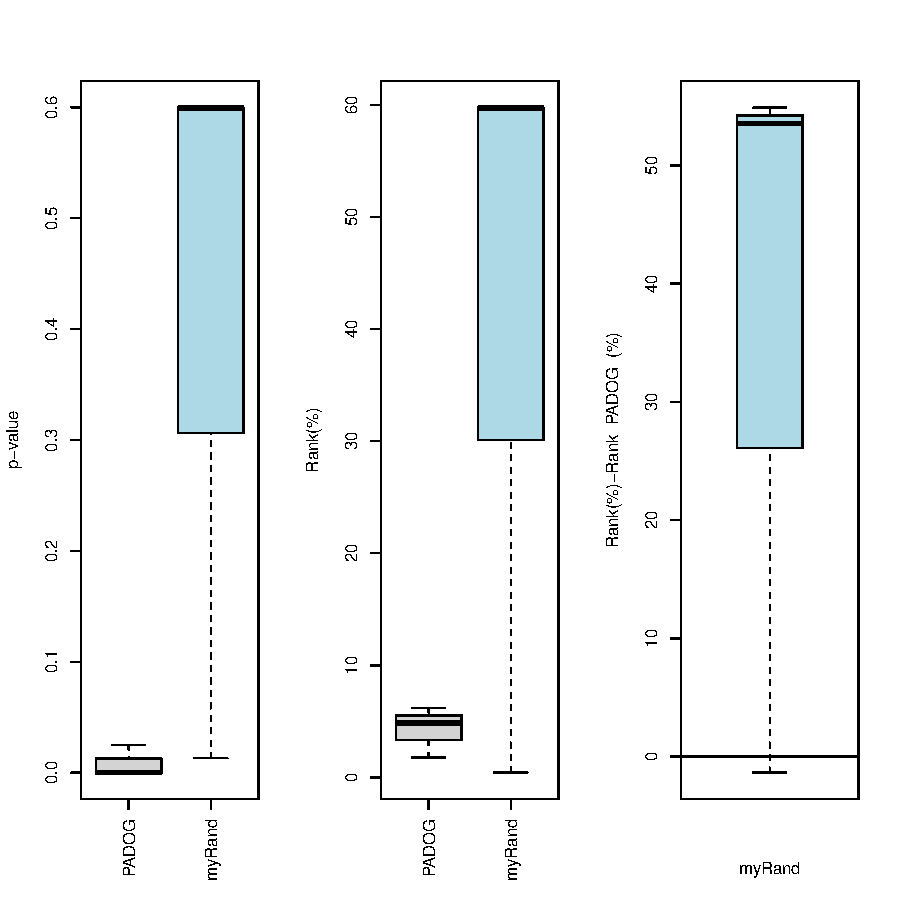
\includegraphics{PADOG-002}

Details about the meaning of the columns in the out table are given in \cite{TarcaPADOG:2012}. The better the
method, the smaller the p-values and ranks for the target pathways, since these are supposted to be 
significant to their respective datasets.  

\bibliography{PADOG} 
\end{document}





